%!TEX root = ../NCVC.tex

\subsection{オプション・ダイアログ全般}
 これまで説明できなかった残りの機能,オプション・ダイアログ全般を系列に分けて記載しています.

\subsubsection{共通}

\begin{minipage}[t]{0.58\textwidth}
1) ツールバーの設定\\
 チェックの入っている所が現在表示されているツールバーです.
カスタマイズボタンを押すと各カテゴリごとにボタンの表示・非表示が切り換えられます.
ツールバーのカスタマイズウィンドウは一般的な Windows アプリケーションと同じなので割愛します.
\end{minipage}
\begin{minipage}[t]{0.02\textwidth}
 
\end{minipage}
\begin{minipage}[t]{0.4\textwidth}
\vspace*{-2zh}
\begin{figure}[H]
\centering
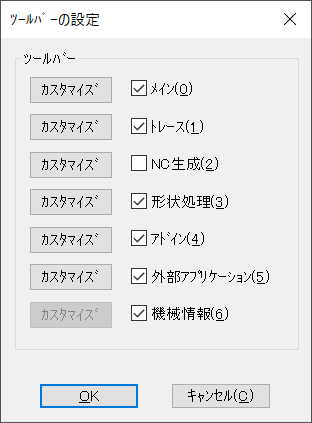
\includegraphics[width=\textwidth]{No6/fig/toolbar.png}
\label{fig:toolbar.png}
\end{figure}
\end{minipage}

\begin{minipage}[t]{0.38\textwidth}
2) 表示属性の設定\\
 まずCAD系・NC系共通の画面属性設定です.
マウスホイールのどちらの向きで拡大縮小するかを設定できます.
\end{minipage}
\begin{minipage}[t]{0.02\textwidth}
 
\end{minipage}
\begin{minipage}[t]{0.6\textwidth}
\vspace*{-2zh}
\begin{figure}[H]
\centering
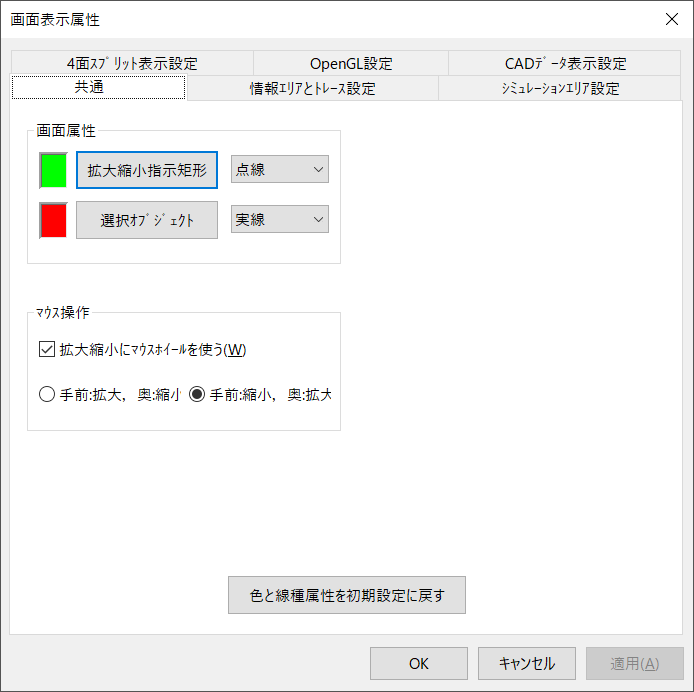
\includegraphics[width=\textwidth]{No6/fig/disp1.png}
\label{fig:disp1.png}
\end{figure}
\end{minipage}

\begin{minipage}[t]{0.38\textwidth}
 NC系加工情報・矩形情報(ウィンドウ左上)の画面属性です.
背景色に違う色を割り当てるとグラデーション表示になります.
Windows98 系ではリソース不足が報告されていますので背景色は同一にして下さい.
ここでトレースのウェイト時間も調整できます.
\end{minipage}
\begin{minipage}[t]{0.02\textwidth}
 
\end{minipage}
\begin{minipage}[t]{0.6\textwidth}
\vspace*{-2zh}
\begin{figure}[H]
\centering
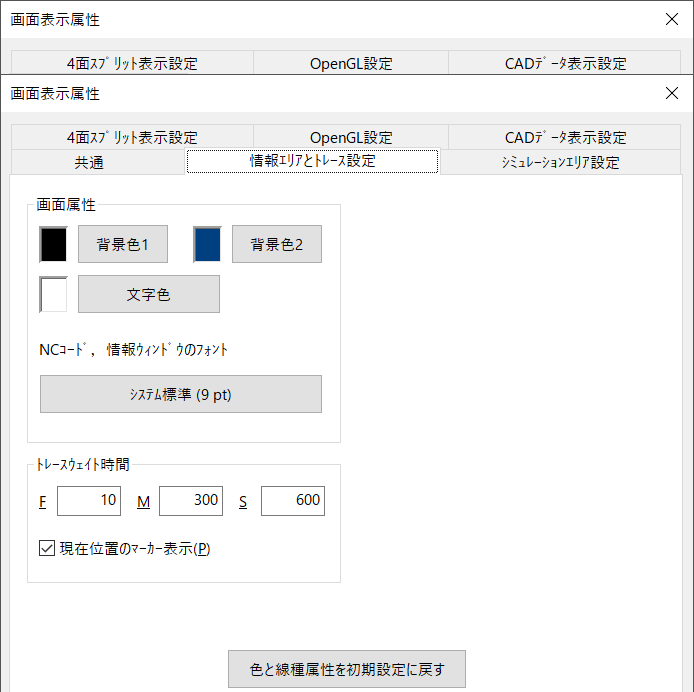
\includegraphics[width=\textwidth]{No6/fig/disp2.png}
\label{fig:disp2.png}
\end{figure}
\end{minipage}

\begin{minipage}[t]{0.38\textwidth}
 NC系メインウィンドウの画面属性です.
\end{minipage}
\begin{minipage}[t]{0.02\textwidth}
 
\end{minipage}
\begin{minipage}[t]{0.6\textwidth}
\vspace*{-2zh}
\begin{figure}[H]
\centering
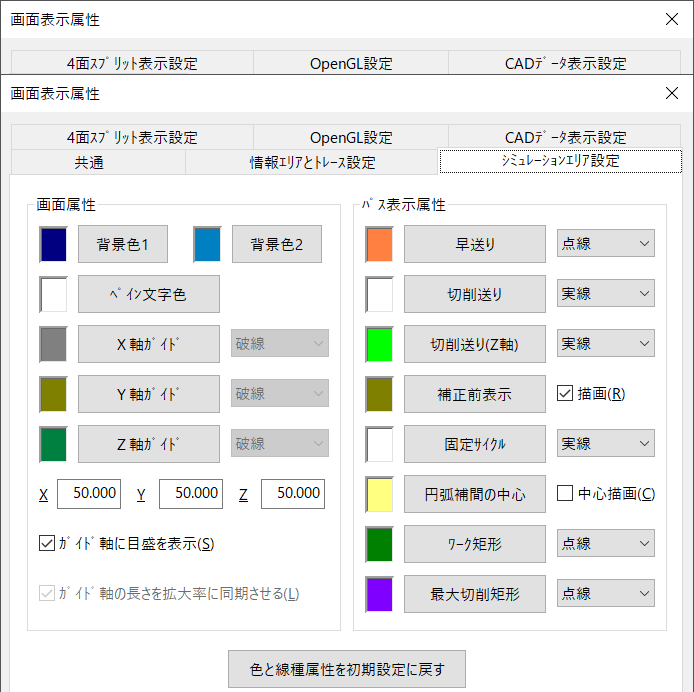
\includegraphics[width=\textwidth]{No6/fig/disp3.png}
\label{fig:disp3.png}
\end{figure}
\end{minipage}

\begin{minipage}[t]{0.38\textwidth}
 
\end{minipage}
\begin{minipage}[t]{0.02\textwidth}
 
\end{minipage}
\begin{minipage}[t]{0.6\textwidth}
\vspace*{-2zh}
\begin{figure}[H]
\centering
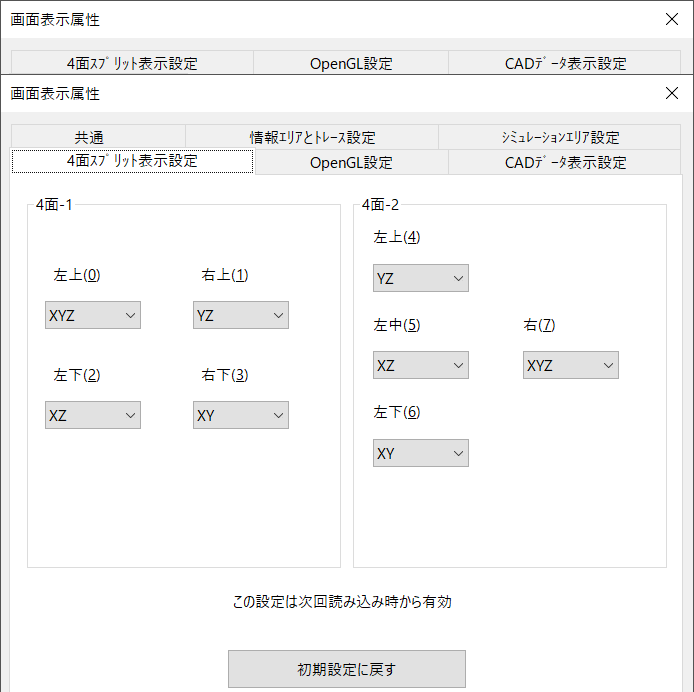
\includegraphics[width=\textwidth]{No6/fig/disp4.png}
\label{fig:disp4.png}
\end{figure}
\end{minipage}

\begin{minipage}[t]{0.38\textwidth}
 
\end{minipage}
\begin{minipage}[t]{0.02\textwidth}
 
\end{minipage}
\begin{minipage}[t]{0.6\textwidth}
\vspace*{-2zh}
\begin{figure}[H]
\centering
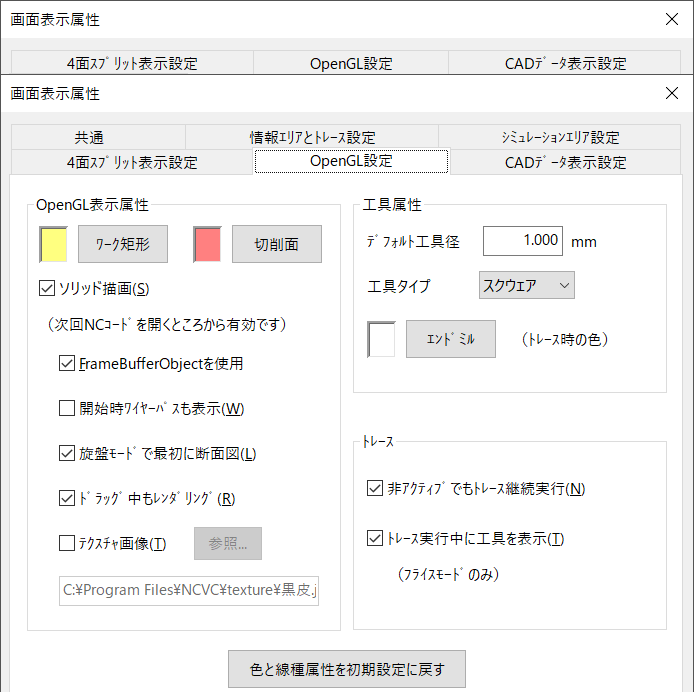
\includegraphics[width=\textwidth]{No6/fig/disp5.png}
\label{fig:disp5.png}
\end{figure}
\end{minipage}

\begin{minipage}[t]{0.38\textwidth}
 CAD系ウィンドウの画面属性です.
NCVC独自に色や線種を割り当てるため,CADでの作図線種や線色は無視されます.
\end{minipage}
\begin{minipage}[t]{0.02\textwidth}
 
\end{minipage}
\begin{minipage}[t]{0.6\textwidth}
\vspace*{-2zh}
\begin{figure}[H]
\centering
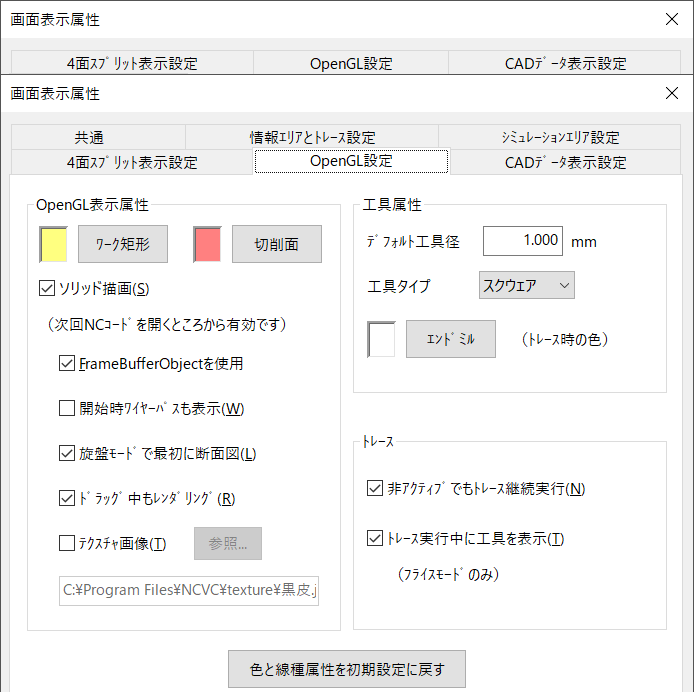
\includegraphics[width=\textwidth]{No6/fig/disp6.png}
\label{fig:disp6.png}
\end{figure}
\end{minipage}

\begin{minipage}[t]{0.38\textwidth}
3) 外部アプリケーションの設定\\
 上側がメニューリスト順,下側が詳細設定です.
詳細設定でプログラムファイル・引数・対象ドキュメントなどを指定し,追加ボタンを押すと上記の一覧に追加されます.
引数に指定できる置換キーワードは以下の通りです.
ただしスペースを含むフォルダ名やファイル名では引数として上手く伝わらない場合があるので必ずダブルクォーテーション(")で括りましょう.
1番目にはテキストエディタを登録しておいて下さい.
[エディタ編集]の場面では1番目の外部アプリケーションが使用されます.
\end{minipage}
\begin{minipage}[t]{0.02\textwidth}
 
\end{minipage}
\begin{minipage}[t]{0.6\textwidth}
\vspace*{-2zh}
\begin{figure}[H]
\centering
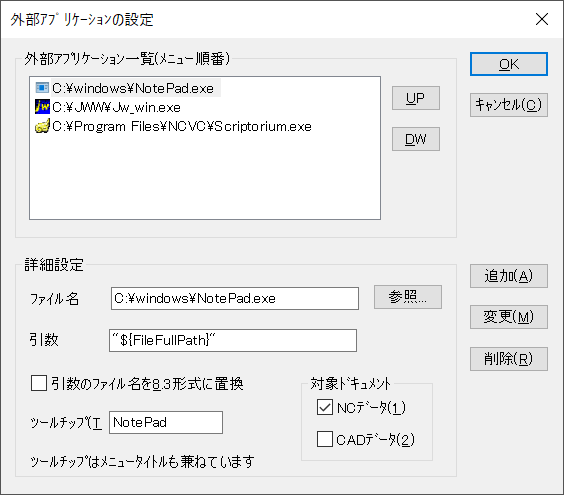
\includegraphics[width=\textwidth]{No6/fig/app.png}
\label{fig:app.png}
\end{figure}
\end{minipage}

\vspace*{2zh}
 ``\,\$\{\,'' と ``\,\}\,'' で括られたとき置換キーワードと認識されます.
\begin{table}[H]
\centering
\begin{tabular}{|p{3cm}|p{10cm}|}
\hline
FileFullPath & 現在アクティブなファイルのフルパス \\ \hline
FilePath     &   〃     ファイルのパス \\ \hline
FileName     &   〃     ファイル名 \\ \hline
FileNameNoExt&   〃     拡張子を除くファイル名 \\ \hline
\end{tabular}
\end{table}

\begin{minipage}[t]{0.48\textwidth}
3) 拡張子の設定\\
 CADデータの拡張子は一般的に定まっていますが,NCファイルの場合は多様です.
しかも中身はテキストファイルなので,システム的にチェックできません.
CAD系・NC系で開く拡張子を登録して下さい.
なお,削除ボタンが有効にならない拡張子は,システム標準かアドインから登録されたものです.
\end{minipage}
\begin{minipage}[t]{0.02\textwidth}
 
\end{minipage}
\begin{minipage}[t]{0.5\textwidth}
\vspace*{-2zh}
\begin{figure}[H]
\centering
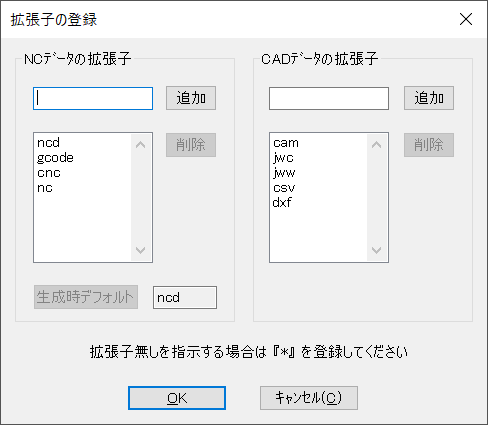
\includegraphics[width=\textwidth]{No6/fig/ext.png}
\label{fig:ext.png}
\end{figure}
\end{minipage}

\subsubsection{CADデータ系}

\begin{minipage}[t]{0.58\textwidth}
1) 原点調整\\
 CADデータを読み込んだあとで原点を動かしたいときに使います.
一時的に変更する場合にだけ使いましょう.
基本的にはCADデータで修正する方をオススメします.
\end{minipage}
\begin{minipage}[t]{0.02\textwidth}
 
\end{minipage}
\begin{minipage}[t]{0.4\textwidth}
\vspace*{-2zh}
\begin{figure}[H]
\centering
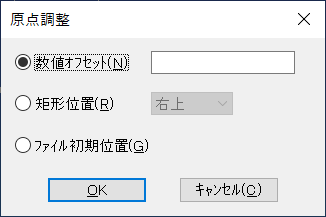
\includegraphics[width=\textwidth]{No6/fig/cad-origin.png}
\label{fig:cad-origin.png}
\end{figure}
\end{minipage}

\begin{minipage}[t]{0.58\textwidth}
2) レイヤ\\
 NCVCで読み込んだレイヤ一覧をツリー形式で表示します.
チェックが入っているレイヤが表示対象であり切削対象でもあります.
単一レイヤのNC生成であってもレイヤが非表示の場合は対象外なのでご注意を.
モードレスダイアログなので,表示しながらNCVC本体の操作が可能です.
\end{minipage}
\begin{minipage}[t]{0.02\textwidth}
 
\end{minipage}
\begin{minipage}[t]{0.4\textwidth}
\vspace*{-2zh}
\begin{figure}[H]
\centering
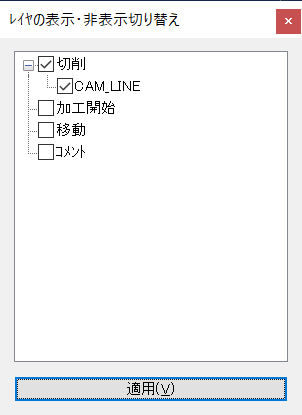
\includegraphics[width=\textwidth]{No6/fig/cad-layer.png}
\label{fig:cad-layer.png}
\end{figure}
\end{minipage}

\subsubsection{NCデータ系}

\begin{minipage}[t]{0.48\textwidth}
1) DXF出力\\
 Gコードのシミュレーション結果をCADデータ(DXF)として出力することができます.
残念ながら3次元データとして出力することはできません.
平面単位(XY, XZ, YZ)の2次元データです.
\end{minipage}
\begin{minipage}[t]{0.02\textwidth}
 
\end{minipage}
\begin{minipage}[t]{0.5\textwidth}
\vspace*{-2zh}
\begin{figure}[H]
\centering
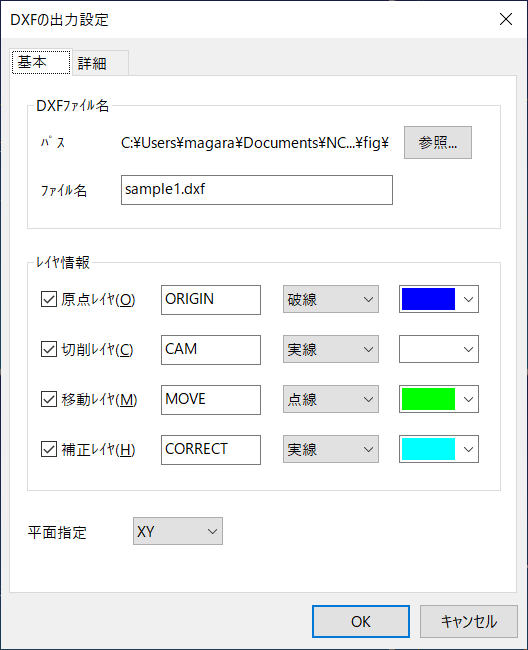
\includegraphics[width=\textwidth]{No6/fig/nc-outdxf.png}
\label{fig:nc-outdxf.png}
\end{figure}
\end{minipage}

\begin{minipage}[t]{0.48\textwidth}
2) ワーク矩形\\
 切削対象となるワークをシミュレーション画面に重ねて表示することができます.
寸法と原点からのオフセットを入力して下さい.
モードレスダイアログなので,表示しながらNCVC本体の操作が可能です.
\end{minipage}
\begin{minipage}[t]{0.02\textwidth}
 
\end{minipage}
\begin{minipage}[t]{0.5\textwidth}
\vspace*{-2zh}
\begin{figure}[H]
\centering
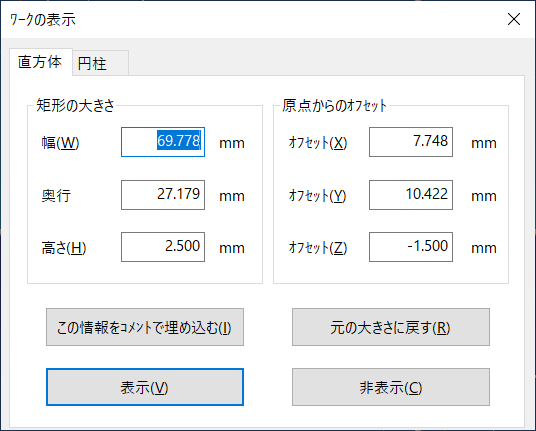
\includegraphics[width=\textwidth]{No6/fig/nc-workrect.png}
\label{fig:nc-workrect.png}
\end{figure}
\end{minipage}

\begin{minipage}[t]{0.58\textwidth}
3) 指定行\\
 Gコードリストの指定された行を表示します.
\end{minipage}
\begin{minipage}[t]{0.02\textwidth}
 
\end{minipage}
\begin{minipage}[t]{0.4\textwidth}
\vspace*{-2zh}
\begin{figure}[H]
\centering
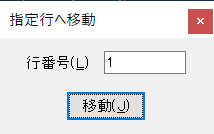
\includegraphics{No6/fig/nc-jump.png}
\label{fig:nc-jump.png}
\end{figure}
\end{minipage}
